\chapter{Methodology}
\label{ch:method}

\section{Prediction task}

The prediction is made at an \emph{index visit}, using only information available at or before that visit. For a participant without dementia at the index visit, the task is to estimate the probability of a clinical diagnosis of dementia within three years:
\begin{equation}
\hat{p} = P\left(\text{dementia diagnosed in } (t_0, t_0 + 3\ \text{years}] \mid \mathbf{x}_{t_0}\right),
\end{equation}
where $t_0$ is the date of the index visit and $\mathbf{x}_{t_0}$ the feature vector at that visit. The main analysis uses each participant's first visit as the index visit. If $T$ denotes the time from $t_0$ to the first visit with a dementia diagnosis and $C$ the time to the last visit, the binary label is
\begin{equation}
y = \begin{cases}
1 & \text{if } T \le 3, \\
0 & \text{if } T > 3 \text{ and } C \ge 3, \\
\text{unknown} & \text{if } T > 3 \text{ and } C < 3,
\end{cases}
\end{equation}
with times in years.

\subsection{Choice of horizon and outcome}

Clinical diagnosis (\texttt{NACCUDSD}) and the Clinical Dementia Rating are recorded at every visit in every form version, which makes them the most consistent outcomes available. A dementia diagnosis was chosen as the main outcome because it is clinically meaningful and easy to interpret. The three-year horizon balances the number of events against loss to follow-up: Kaplan--Meier estimates \cite{kaplan1958} show that about 35\% of participants with MCI progress to dementia within three years, and that 11\% of cognitively normal participants progress to MCI or dementia, while the number of participants with a known status falls steadily with longer horizons and most PET scans are too recent for a five-year horizon. The Kaplan--Meier estimate of the probability of remaining free of the event up to time $t$ is
\begin{equation}
\hat{S}(t) = \prod_{t_i \le t} \left(1 - \frac{d_i}{n_i}\right),
\end{equation}
where $d_i$ is the number of events at time $t_i$ and $n_i$ the number of participants still under observation just before $t_i$; the three-year progression rate is $1 - \hat{S}(3)$ (Figure~\ref{fig:km}).

\begin{figure}[H]
\centering
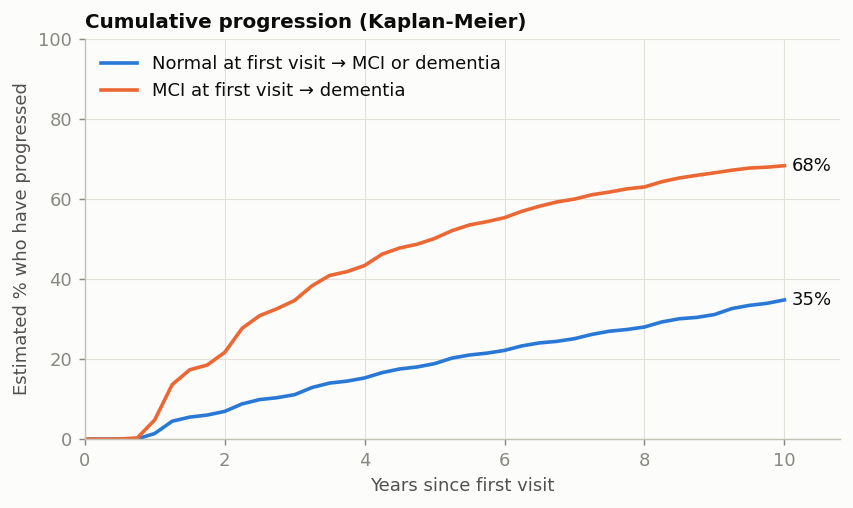
\includegraphics[width=0.75\textwidth]{02_progression_curves.png}
\caption{Kaplan--Meier estimates of cumulative progression from the first visit: cognitively normal participants to MCI or dementia, and participants with MCI to dementia.}
\label{fig:km}
\end{figure}


\subsection{Censoring}

A participant last seen less than three years after the index visit without a dementia diagnosis has an unknown outcome. Such participants were excluded from the binary task rather than counted as negative, which would bias the estimated risk downwards. Because this exclusion could itself introduce bias, a Cox proportional hazards model \cite{cox1972} that uses all eligible participants, including the censored ones, was fitted as a robustness check (Section~\ref{sec:res_sens}). Figure~\ref{fig:outcome} illustrates the three possible cases.

\begin{figure}[H]
\centering
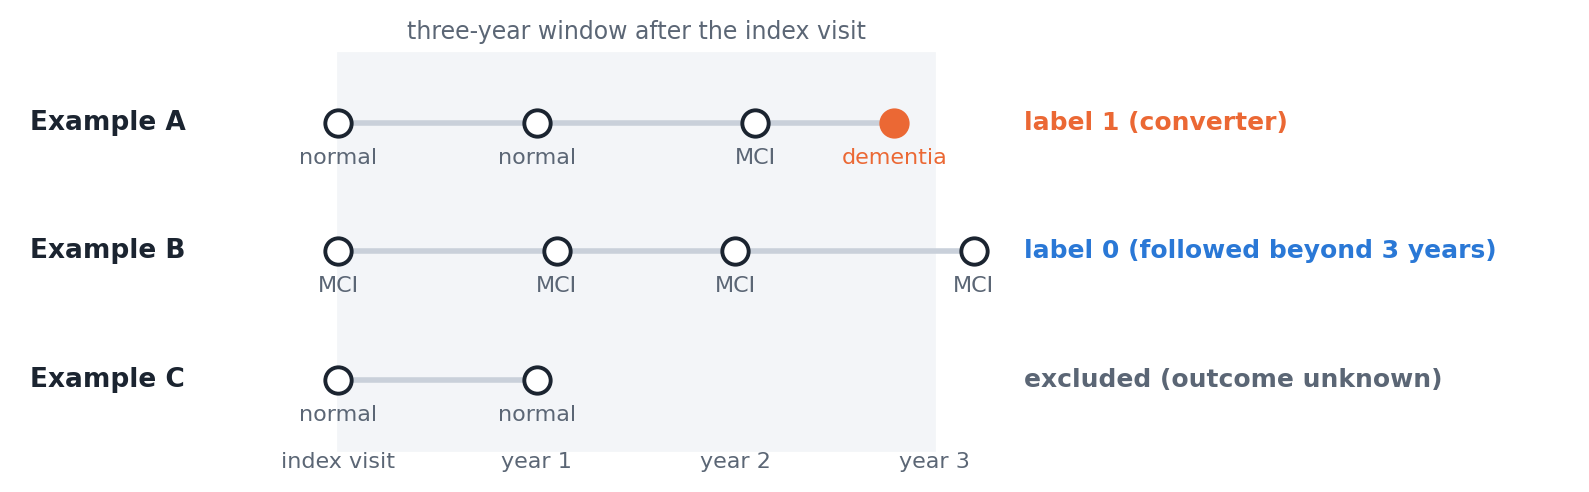
\includegraphics[width=\textwidth]{outcome.png}
\caption{Definition of the outcome. Only the index visit supplies features; later visits supply the label.}
\label{fig:outcome}
\end{figure}

\subsection{Secondary outcomes: cognitive decline}

Dementia is one end point of cognitive decline, but many people worsen without reaching it. Two further outcomes were therefore defined from the CDR Sum of Boxes, which is recorded at every visit in every form version. The binary decline outcome is a rise of at least one point in CDR-SB at any visit within three years of the index visit; it is unknown for participants who neither rose by a point nor were followed for three years. The continuous progression outcome is the change in CDR-SB between the index visit and the visit closest to three years later, accepted if that visit falls within six months of the three-year mark. Writing $c(t)$ for CDR-SB at time $t$ after the index visit and $v_i$ for the visit times,
\begin{equation}
y_{\text{dec}} = \mathbb{1}\Big[\max_{0 < v_i \le 3} c(v_i) - c(0) \ge 1\Big],
\qquad
\Delta = c(v^{*}) - c(0), \quad v^{*} = \operatorname*{arg\,min}_{|v_i - 3| \le 0.5} |v_i - 3|.
\end{equation}
The same eligibility rules and splits are used for all outcomes.

\section{Cohort}

Table~\ref{tab:flow} shows how the cohort was formed. Visits had to be in person, because telephone visits lack the neuropsychological tests, and on form versions 1 to 3, because version~4 reorganised many of the other variables and accounts for only 3\% of visits. Participants with dementia at the index visit, or at any earlier visit, are not eligible.

\begin{table}[H]
\centering\small
\caption{Cohort flow.}
\label{tab:flow}
\begin{tabular}{@{}lr@{}}
\toprule
Step & Participants \\
\midrule
All participants & 57,038 \\
First visit in person, form version 1 to 3 & 55,461 \\
\quad and not demented at that visit & 38,107 \\
\quad and outcome known at three years & 19,470 \\
\quad\quad of whom diagnosed with dementia within three years & 2,818 (14.5\%) \\
\bottomrule
\end{tabular}
\end{table}

The ``not demented'' cohort contains three clinically different groups: 12,377 cognitively normal participants (198 converters, 1.6\%), 5,993 participants with MCI (2,485 converters, 41.5\%) and 1,100 participants classed as impaired but not MCI (135 converters, 12.3\%). Results are reported for the whole cohort and for the normal and MCI groups separately.

\section{Feature construction}

\subsection{Harmonised cognitive scores}
\label{sec:zscores}

To place tests from different form versions on one scale, each raw score $s$ was converted into a demographically adjusted $z$-score. For each test, a linear model of the score on age, sex and education was fitted among cognitively normal participants at their first visit, using the training set only:
\begin{equation}
\hat{s} = \beta_0 + \beta_1\,\text{age} + \beta_2\,\text{female} + \beta_3\,\text{education},
\qquad
z = \frac{s - \hat{s}}{\sigma_{\text{res}}},
\end{equation}
where $\sigma_{\text{res}}$ is the residual standard deviation of the fitted model. The sign is reversed for the two timed Trail Making tests, so that a negative $z$ always means worse than expected. Values were clipped to $[-5, 5]$. The $z$-scores of the tests in one cognitive domain were then averaged to give six domain scores: global screening (MoCA, MMSE), memory, attention, speed and executive function, language, and visuospatial function. A participant receives a domain score from whichever tests their visit contained.

As an example, for the MoCA the fitted model is $\hat{s} = 23.0 - 0.059\,\text{age} + 0.33\,\text{female} + 0.42\,\text{education}$ with $\sigma_{\text{res}} = 2.56$, estimated from 6,264 normal participants. A 72-year-old woman with 16 years of education has an expected score of 25.8, so a score of 21 corresponds to $z = -1.9$ (Figure~\ref{fig:zscore}).

\begin{figure}[H]
\centering
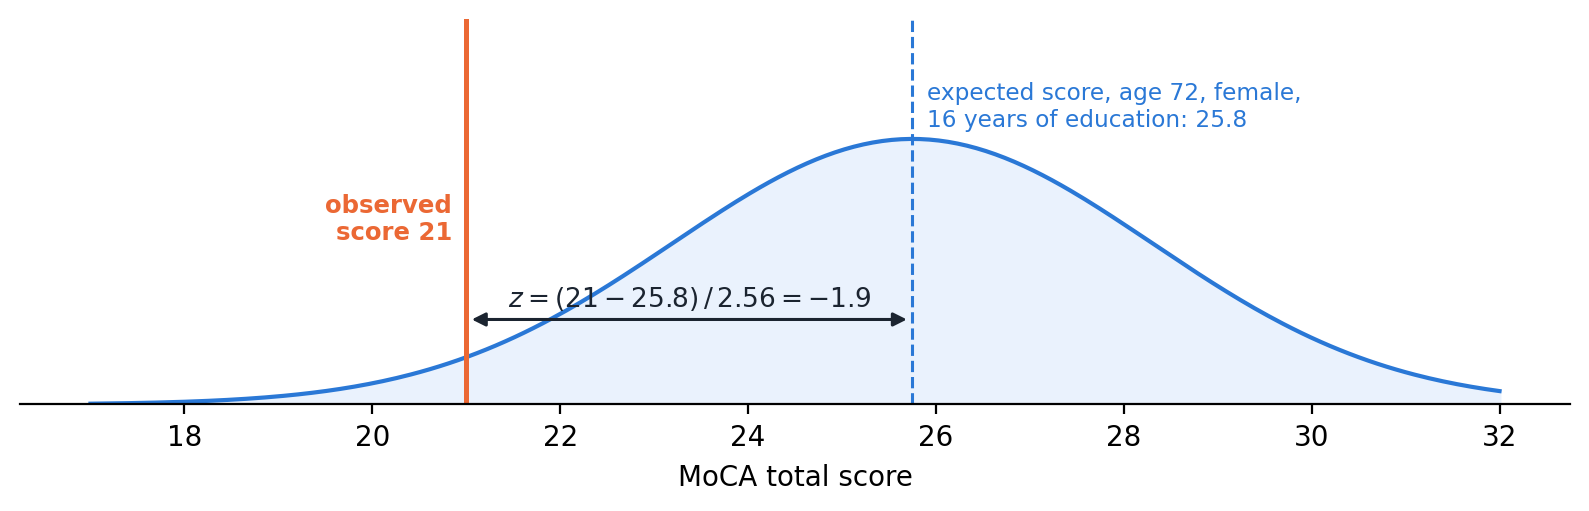
\includegraphics[width=\textwidth]{zscore.png}
\caption{Demographically adjusted $z$-score for the MoCA, using the fitted normative model.}
\label{fig:zscore}
\end{figure}

The harmonisation was checked on cognitively normal participants who were not used to fit the norms: their mean domain $z$-scores lie within 0.1 of zero under every form version, while participants with MCI and dementia score progressively lower (Figure~\ref{fig:harmon}). The scores therefore mean the same thing whichever tests a visit contained.

\begin{figure}[H]
\centering
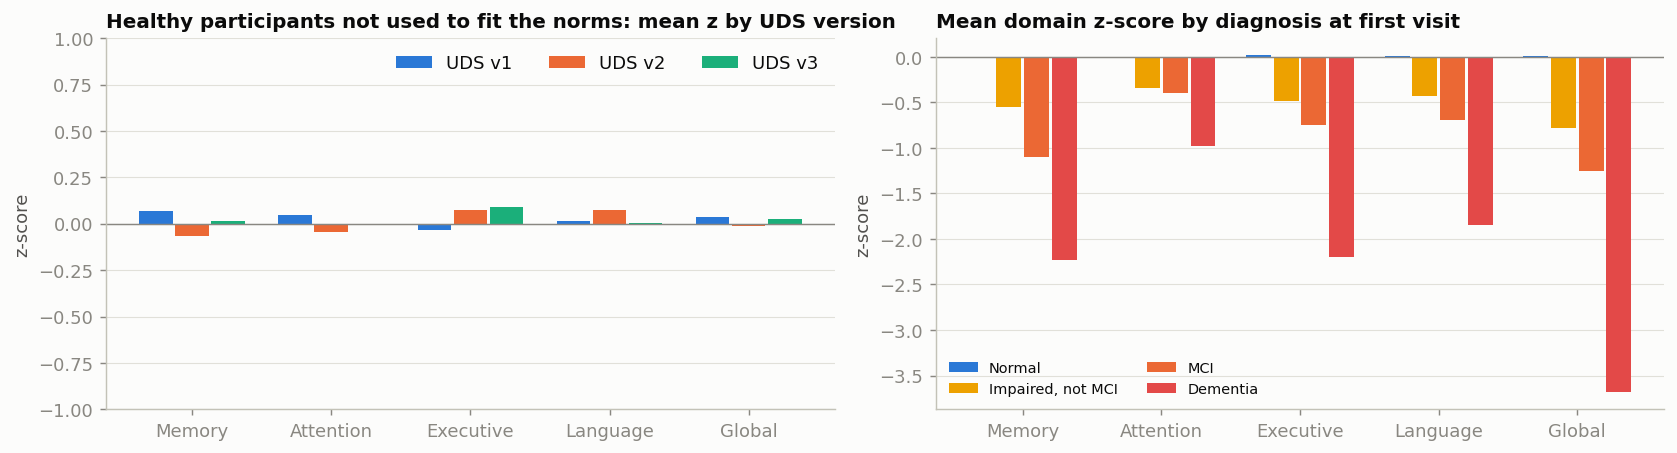
\includegraphics[width=\textwidth]{05_cognitive_harmonisation.png}
\caption{Left: mean domain $z$-score of cognitively normal participants not used to fit the norms, by UDS version. Right: mean domain $z$-score by diagnosis at the first visit.}
\label{fig:harmon}
\end{figure}


Three further cognitive features were derived: the number of tests the participant could not complete for cognitive or behavioural reasons (NACC code 96 or 996), which is informative about severity and is therefore kept rather than treated as missing; the Geriatric Depression Scale total; and the number of NPI-Q behavioural symptoms present.

\subsection{Cardiovascular history}

Each condition $k$ was coded as ``ever present'', $h_k(t) = \max_{v_i \le t} r_k(v_i)$, where $r_k(v_i) = 1$ if the condition is recorded at visit $v_i$. The record was taken from the participant-reported history (form A5, where both recent and remote mentions count) and, where that form was blank, from the clinician-assessed form D2. Once present, a condition remains present at all later visits. Measured blood pressure, heart rate and BMI use the most recent measurement up to the visit. Two summary features were derived: pulse pressure, $\text{PP} = \text{BP}_{\text{sys}} - \text{BP}_{\text{dia}}$, and the vascular risk count, $R = h_{\text{HTN}} + h_{\text{chol}} + h_{\text{DM}} + h_{\text{smoke}} \in \{0, \dots, 4\}$.

\subsection{Genetics}

The number of APOE $\varepsilon$4 alleles is used directly. About one participant in five was not genotyped; genotyping depends on centre and consent and is therefore not random, so these participants receive a separate ``not genotyped'' indicator instead of an imputed value.

\subsection{Preventing the use of future information}
\label{sec:pettiming}

No feature at a visit may depend on a later visit. Fixed characteristics such as education are carried forward from the visit where they were first recorded, never backwards. A PET scan is used at a visit only if it was acquired on or up to 365 days before that visit. Both rules were introduced after the verification step described in Chapter~\ref{ch:verification} found violations in an earlier version of the pipeline.

\section{Data splits}

All splits were made at participant level, so that all visits of a person fall in the same partition. Twenty percent of the centres (9 of 46) were held out entirely to measure performance at sites the model has never seen. The remaining participants were divided into training (70\%), validation (15\%) and test (15\%) sets, stratified by diagnosis at the first visit. The random seed was fixed (2026). Table~\ref{tab:splits} gives the resulting sizes for the first-visit cohort.

\begin{table}[H]
\centering\small
\caption{Partition sizes for the main cohort.}
\label{tab:splits}
\begin{tabular}{@{}lrr@{}}
\toprule
Partition & Participants & Converters \\
\midrule
Training & 10,879 & 1,599 \\
Validation & 2,241 & 342 \\
Test & 2,286 & 332 \\
Held-out centres & 4,064 & 545 \\
\bottomrule
\end{tabular}
\end{table}

\begin{figure}[H]
\centering
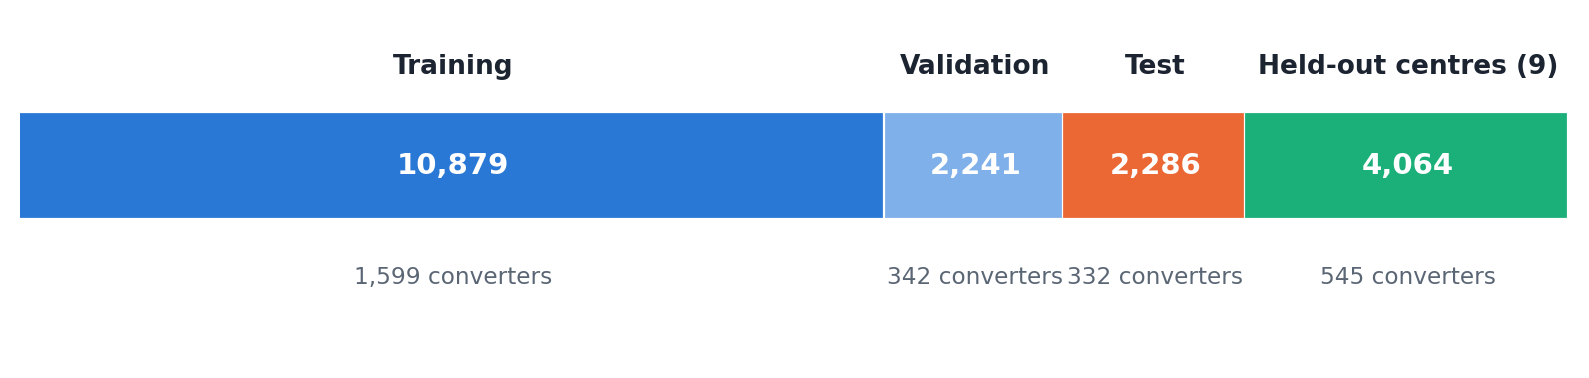
\includegraphics[width=\textwidth]{split.png}
\caption{Participant-level partitions of the main cohort.}
\label{fig:split}
\end{figure}

Every quantity estimated from data (normative models for $z$-scores, tau standardisation, imputation medians, scaling) was fitted on the training set and applied unchanged to the other sets. The validation set was used for early stopping and model selection; the test set and the held-out centres were used only for evaluation.

\section{Models}

Five classifiers of increasing complexity were compared on the same 48 features (Table~\ref{tab:models}); their mathematical form is given in Section~\ref{sec:model_maths}. Logistic regression is the standard baseline in clinical prediction. Random forests \cite{breiman2001} and gradient-boosted trees (XGBoost \cite{chen2016}) are strong learners for tabular data that handle non-linear effects and interactions. A multilayer perceptron and the FT-Transformer \cite{gorishniy2021} represent deep learning; the latter tokenises each feature and applies self-attention, and is among the strongest deep architectures reported for tabular data. Except for logistic regression, every model was trained with three random seeds and the predictions were averaged.

\begin{table}[H]
\centering\small
\caption{Models and settings.}
\label{tab:models}
\begin{tabularx}{\textwidth}{@{}lY@{}}
\toprule
Model & Settings \\
\midrule
Logistic regression & Median imputation with missing-value indicators, standardisation; regularisation strength chosen from five values on the validation set \\
Random forest & 500 trees, minimum 10 samples per leaf, $\sqrt{p}$ features per split \\
XGBoost & Up to 3,000 trees, learning rate 0.03, depth chosen from \{3, 4, 6\} on validation AUROC, subsample and column sample 0.8, early stopping after 100 rounds without improvement; missing values handled natively \\
Multilayer perceptron & Two hidden layers (128 and 64 units), dropout 0.2, AdamW, early stopping on validation AUROC \\
FT-Transformer & Feature tokens of dimension 64, three Transformer layers with eight heads, a learned token for each missing feature, early stopping on validation AUROC \\
\bottomrule
\end{tabularx}
\end{table}

XGBoost was used as the main model for all further experiments because it performed as well as the others, handles missing values without imputation and allows exact Shapley value explanations. For the progression outcome, the same gradient-boosting settings were used with an absolute-error objective, and the model was compared with the simplest reference, predicting no change.

\subsection{Mathematical form of the models}
\label{sec:model_maths}

Let $\mathbf{x} \in \mathbb{R}^{p}$ be the feature vector of a participant, $y \in \{0,1\}$ the label and $\sigma(u) = 1/(1+e^{-u})$ the logistic function. All classifiers output a probability $\hat{p} = \sigma(f(\mathbf{x}))$ and, apart from the random forest, are fitted by minimising the binary cross-entropy over the $n$ training participants,
\begin{equation}
\mathcal{L}_{\text{BCE}} = -\frac{1}{n} \sum_{i=1}^{n} \Big[ y_i \log \hat{p}_i + (1 - y_i) \log (1 - \hat{p}_i) \Big],
\label{eq:bce}
\end{equation}
plus a model-specific penalty.

\paragraph{Logistic regression.} After median imputation, missing-value indicators and standardisation give a vector $\tilde{\mathbf{x}}$, the model is $f(\mathbf{x}) = \beta_0 + \boldsymbol{\beta}^{\top}\tilde{\mathbf{x}}$ with an $L_2$ penalty,
\begin{equation}
\min_{\beta_0, \boldsymbol{\beta}} \; \frac{1}{2}\lVert \boldsymbol{\beta} \rVert_2^2 + C \sum_{i=1}^{n} \ell(y_i, \hat{p}_i), \qquad C \in \{0.01, 0.03, 0.1, 0.3, 1\},
\end{equation}
where $\ell$ is the per-participant cross-entropy and $C$ was chosen on the validation set.

\paragraph{Random forest.} The forest averages the class-probability estimates of $B = 500$ decision trees, each grown on a bootstrap sample with $\lfloor\sqrt{p}\rfloor$ candidate features per split: $\hat{p}(\mathbf{x}) = \frac{1}{B}\sum_{b=1}^{B} \hat{p}_b(\mathbf{x})$.

\paragraph{Gradient-boosted trees (XGBoost).} The score is a sum of regression trees, built one at a time:
\begin{equation}
f_M(\mathbf{x}) = \sum_{m=1}^{M} \eta\, g_m(\mathbf{x}), \qquad \eta = 0.03.
\end{equation}
Tree $g_m$ is chosen to minimise a second-order approximation of the regularised objective
\begin{equation}
\sum_{i=1}^{n} \Big[ G_i\, g_m(\mathbf{x}_i) + \tfrac{1}{2} H_i\, g_m(\mathbf{x}_i)^2 \Big] + \gamma J + \tfrac{1}{2}\lambda \sum_{j=1}^{J} w_j^2,
\end{equation}
where $G_i = \hat{p}_i - y_i$ and $H_i = \hat{p}_i(1 - \hat{p}_i)$ are the first and second derivatives of the loss at the current model, $J$ is the number of leaves, $w_j$ the leaf values, $\lambda = 2$ and $\gamma = 0$. For a leaf containing the participant set $I_j$ the optimal value is $w_j^{*} = -\sum_{i \in I_j} G_i / (\sum_{i \in I_j} H_i + \lambda)$, and a split is kept only if every child has $\sum H_i \ge 5$ (minimum child weight). Missing values are sent down a default branch learned from the data. For the progression outcome the loss is the absolute error $\lvert \Delta_i - f(\mathbf{x}_i) \rvert$, whose minimiser is the conditional median.

\paragraph{Multilayer perceptron.} With $\tilde{\mathbf{x}}$ as for logistic regression,
\begin{equation}
\mathbf{h}_1 = \operatorname{ReLU}(\mathbf{W}_1 \tilde{\mathbf{x}} + \mathbf{b}_1), \quad
\mathbf{h}_2 = \operatorname{ReLU}(\mathbf{W}_2 \mathbf{h}_1 + \mathbf{b}_2), \quad
f(\mathbf{x}) = \mathbf{w}_3^{\top} \mathbf{h}_2 + b_3,
\end{equation}
with 128 and 64 hidden units and dropout of 0.2 after each hidden layer.

\paragraph{FT-Transformer.} Each feature $j$ becomes a token $\mathbf{e}_j = x_j \mathbf{w}_j + \mathbf{b}_j \in \mathbb{R}^{64}$, or a learned token $\mathbf{m}_j$ when $x_j$ is missing. A learned classification token $\mathbf{e}_0$ is prepended, and three pre-norm Transformer layers are applied. Each layer computes multi-head self-attention,
\begin{equation}
\operatorname{Attn}(\mathbf{Q}, \mathbf{K}, \mathbf{V}) = \operatorname{softmax}\!\left( \frac{\mathbf{Q}\mathbf{K}^{\top}}{\sqrt{d_k}} \right) \mathbf{V},
\end{equation}
with eight heads ($d_k = 8$), followed by a feed-forward block with GELU activation; both have residual connections. The output for $\mathbf{e}_0$ passes through layer normalisation and a linear layer to give $f(\mathbf{x})$.

Both networks were trained with AdamW (learning rate $10^{-3}$ for the perceptron and $5 \times 10^{-4}$ for the FT-Transformer, weight decay $10^{-4}$) on batches of 256, and training stopped when the validation AUROC had not improved for eight epochs.

\section{Modality-Encoder Fusion Network}
\label{sec:fusion_net}

To test the fusion architecture proposed at the start of the project, a neural network was built in which each of the five kinds of information has its own encoder. Each encoder is a two-layer network that maps the features of one modality to a 32-dimensional token. When a modality is entirely missing for a participant, its token is replaced by a learned ``missing'' token, so the network can tell an absent modality from a normal one. A learned type embedding identifies each modality. A four-head attention layer, queried by a learned summary vector, combines the five tokens into one representation (Tier~1 fusion), and the attention weights show how much the network drew on each modality. Two heads share this representation: a risk head for dementia within three years and a progression head for the three-year change in CDR-SB, trained jointly with a binary cross-entropy loss and a Huber loss weighted by 0.5 on the participants with a known change. Modality dropout with probability 0.35 was applied during training. The network was trained with AdamW (learning rate $10^{-3}$), early stopping on validation AUROC, and three seeds whose predictions were averaged. PET measures are added afterwards by the late-fusion model (Tier~2), because too few scanned participants have three-year outcomes to train them inside the network.

Formally, let $\mathbf{x}^{(g)}$ be the features of modality $g \in \{1, \dots, 5\}$ and $\pi_g \in \{0, 1\}$ indicate whether the modality is present. The token of modality $g$ is
\begin{equation}
\mathbf{t}_g = \pi_g\, E_g\big(\mathbf{x}^{(g)}\big) + (1 - \pi_g)\, \mathbf{m}_g + \boldsymbol{\tau}_g, \qquad
E_g(\mathbf{x}) = \mathbf{W}_{g2}\, \operatorname{ReLU}(\mathbf{W}_{g1}\mathbf{x} + \mathbf{b}_{g1}) + \mathbf{b}_{g2},
\end{equation}
where $\mathbf{m}_g$ is the learned missing token and $\boldsymbol{\tau}_g$ the type embedding, all in $\mathbb{R}^{32}$. For each attention head $h$, the learned query $\mathbf{q}$ gives the weights
\begin{equation}
\alpha_{g}^{(h)} = \frac{\exp\big( (\mathbf{W}^{(h)}_Q \mathbf{q})^{\top} \mathbf{W}^{(h)}_K \mathbf{t}_g / \sqrt{8} \big)}{\sum_{g'} \exp\big( (\mathbf{W}^{(h)}_Q \mathbf{q})^{\top} \mathbf{W}^{(h)}_K \mathbf{t}_{g'} / \sqrt{8} \big)}, \qquad
\mathbf{z} = \operatorname{LN}\Big( \mathbf{W}_O \big[ \textstyle\sum_g \alpha^{(h)}_g \mathbf{W}^{(h)}_V \mathbf{t}_g \big]_{h=1}^{4} \Big),
\end{equation}
and the reported attention share of modality $g$ is the average of $\alpha^{(h)}_g$ over the four heads. The risk head gives $\hat{p} = \sigma(r(\mathbf{z}))$ and the progression head $\hat{\Delta} = q(\mathbf{z})$, each a two-layer network. The training loss is
\begin{equation}
\mathcal{L} = \mathcal{L}_{\text{BCE}} + 0.5\, \frac{1}{|\mathcal{D}_\Delta|} \sum_{i \in \mathcal{D}_\Delta} \rho\big(\Delta_i - \hat{\Delta}_i\big), \qquad
\rho(u) = \begin{cases} \tfrac{1}{2}u^2 & |u| \le 1, \\ |u| - \tfrac{1}{2} & |u| > 1, \end{cases}
\end{equation}
where $\mathcal{D}_\Delta$ is the set of participants in the batch whose three-year change is known and $\rho$ is the Huber loss. Gradients were clipped to a norm of 1.

\section{Contribution of each feature category}

The contribution of a category was measured by ablation: the model was trained with all categories and again without the category of interest, and the paired difference in AUROC on the same participants was computed with bootstrap confidence intervals,
\begin{equation}
\Delta\text{AUROC}_{\mathcal{G}} = \text{AUROC}\big(f_{\text{all}}\big) - \text{AUROC}\big(f_{\text{all} \setminus \mathcal{G}}\big).
\end{equation} Each category was also evaluated alone and in cumulative order.

\section{Longitudinal models}

To test whether earlier visits add information, the index visit was moved to a later ``landmark'' visit preceded by at least two earlier visits. Three models were compared on the same landmarks: XGBoost on the landmark visit only; XGBoost with slope and change features of the cognitive scores and CDR-SB over the earlier visits; and a gated recurrent unit (GRU) \cite{cho2014} with 48 hidden units that reads up to six visits, with the time of each visit as an input because visit intervals are irregular. For visit $k$ with input $\mathbf{s}_k$ (standardised scores, missing-value flags and years before the landmark), the GRU updates its state as
\begin{align}
\mathbf{r}_k &= \sigma(\mathbf{W}_r \mathbf{s}_k + \mathbf{U}_r \mathbf{h}_{k-1} + \mathbf{b}_r), &
\mathbf{u}_k &= \sigma(\mathbf{W}_u \mathbf{s}_k + \mathbf{U}_u \mathbf{h}_{k-1} + \mathbf{b}_u), \nonumber\\
\tilde{\mathbf{h}}_k &= \tanh\big(\mathbf{W}_h \mathbf{s}_k + \mathbf{U}_h (\mathbf{r}_k \odot \mathbf{h}_{k-1}) + \mathbf{b}_h\big), &
\mathbf{h}_k &= (1 - \mathbf{u}_k) \odot \tilde{\mathbf{h}}_k + \mathbf{u}_k \odot \mathbf{h}_{k-1},
\end{align}
and the final state is joined with a 96-unit encoding of the landmark-visit features before a small output network. The trajectory features for XGBoost are, for each score, the least-squares slope over the visits up to the landmark, $\hat{b} = \sum_k (\tau_k - \bar{\tau})(s_k - \bar{s}) / \sum_k (\tau_k - \bar{\tau})^2$ with visit times $\tau_k$, and the change since the previous visit.

\section{PET late fusion}

Because few scanned participants have three years of follow-up, a large model cannot be fitted on PET participants alone. A late-fusion design was used: the clinical model, trained on all participants, produces a risk $\hat{p}_{\text{clin}}$ for each scanned participant; a small, strongly regularised logistic regression then combines the logit of that risk with the PET measures $\mathbf{u}$ and indicators $\boldsymbol{\delta}$ of which measures are present:
\begin{equation}
\operatorname{logit} \hat{p}_{\text{PET}} = \gamma_0 + \gamma_1 \log\frac{\hat{p}_{\text{clin}}}{1 - \hat{p}_{\text{clin}}} + \boldsymbol{\gamma}_u^{\top}\mathbf{u} + \boldsymbol{\gamma}_\delta^{\top}\boldsymbol{\delta}.
\end{equation}
Because few events are available, the $L_2$ penalty was set firmly ($C = 0.3$ in the final model). Two rules for matching scans to visits were compared: a strict rule (scan on or before the index visit) and a nearest-visit rule (larger, but the scan may follow the visit by a few weeks).

\section{Modality dropout}

In practice not every patient has every assessment. A model trained on complete records may behave poorly when an entire category is missing. To make one model usable with any combination of available information, the training data were augmented with four additional copies in which each optional category (genetics, cardiovascular, cognitive tests, clinical stage) was removed independently with probability 0.35. For copy $k$ of participant $i$ and optional category $g$,
\begin{equation}
\tilde{\mathbf{x}}^{(g)}_{ik} = \begin{cases} \text{missing} & \text{if } \xi_{ikg} = 1, \\ \mathbf{x}^{(g)}_i & \text{otherwise}, \end{cases} \qquad \xi_{ikg} \sim \operatorname{Bernoulli}(0.35),
\end{equation}
so that the model sees every pattern of missing categories during training, while demographics are always kept. This model was compared with a standard model and with specialist models retrained for each pattern of missing categories.

\section{Explainability}

Predictions were explained with Shapley additive explanations (SHAP) \cite{lundberg2017}, computed exactly for the tree ensemble with TreeSHAP \cite{lundberg2020}. For each test participant, SHAP decomposes the predicted log-odds into a sum of feature contributions,
\begin{equation}
f(\mathbf{x}) = \phi_0 + \sum_{j=1}^{p} \phi_j, \qquad
\phi_j = \sum_{S \subseteq F \setminus \{j\}} \frac{|S|!\,(p - |S| - 1)!}{p!} \Big[ f_{S \cup \{j\}}(\mathbf{x}) - f_S(\mathbf{x}) \Big],
\end{equation}
where $F$ is the set of all features, $f_S$ the expected model output when only the features in $S$ are known, and $\phi_0$ the average output over the training data. Global importance is the mean absolute contribution of a feature over the test set, $I_j = \frac{1}{n}\sum_i |\phi_{ij}|$; the importance of a category $\mathcal{G}$ is $\sum_{j \in \mathcal{G}} I_j$, reported as a share of $\sum_j I_j$. Stability was assessed by refitting the model on eight bootstrap samples of the training set.

\section{Evaluation}

Discrimination was measured by the area under the ROC curve (AUROC) and the area under the precision--recall curve (AUPRC). The AUROC equals the probability that a randomly chosen converter receives a higher predicted risk than a randomly chosen non-converter,
\begin{equation}
\text{AUROC} = \frac{1}{n_1 n_0} \sum_{i: y_i = 1} \sum_{j: y_j = 0} \Big( \mathbb{1}[\hat{p}_i > \hat{p}_j] + \tfrac{1}{2}\mathbb{1}[\hat{p}_i = \hat{p}_j] \Big),
\end{equation}
where $n_1$ and $n_0$ are the numbers of converters and non-converters. The AUPRC was computed as average precision, $\sum_k (R_k - R_{k-1}) P_k$, over the thresholds $k$ with precision $P_k$ and recall $R_k$; for an uninformative model it equals the event rate.

Calibration was assessed by the Brier score, the calibration slope and intercept, and by comparing predicted and observed risk in deciles:
\begin{equation}
B = \frac{1}{n}\sum_{i=1}^{n} (\hat{p}_i - y_i)^2, \qquad
\operatorname{logit} P(y_i = 1) = a + b\, \operatorname{logit} \hat{p}_i,
\end{equation}
where $a$ and $b$ are estimated by logistic regression; a well-calibrated model has $b = 1$ and $a = 0$. A constant prediction equal to the event rate $\pi$ has $B = \pi(1 - \pi)$, which is the reference value quoted with the results.

Clinical usefulness was assessed by decision curve analysis \cite{vickers2006} and by sensitivity, specificity and predictive values at fixed risk thresholds. At a threshold $t$, where a participant is flagged if $\hat{p} \ge t$, the net benefit is
\begin{equation}
\text{NB}(t) = \frac{\text{TP}(t)}{n} - \frac{\text{FP}(t)}{n} \cdot \frac{t}{1 - t},
\end{equation}
which counts true positives and penalises false positives by the odds of the threshold. It is compared with flagging everyone, $\text{NB}_{\text{all}}(t) = \pi - (1 - \pi)\, t/(1 - t)$, and with flagging no one ($\text{NB} = 0$), for $t$ from 0.02 to 0.60. Sensitivity is $\text{TP}/(\text{TP} + \text{FN})$, specificity $\text{TN}/(\text{TN} + \text{FP})$, positive predictive value $\text{TP}/(\text{TP} + \text{FP})$ and negative predictive value $\text{TN}/(\text{TN} + \text{FN})$.

For the progression outcome, the mean absolute error $\text{MAE} = \frac{1}{n}\sum_i |\Delta_i - \hat{\Delta}_i|$, the coefficient of determination $R^2 = 1 - \sum_i (\Delta_i - \hat{\Delta}_i)^2 / \sum_i (\Delta_i - \bar{\Delta})^2$ and the Spearman rank correlation were reported, each against the reference $\hat{\Delta} = 0$.

Uncertainty was quantified by $R = 1{,}000$ bootstrap resamples of the evaluation set. For a statistic $\theta$, the 95\% interval is $[\theta^{*}_{(0.025)}, \theta^{*}_{(0.975)}]$, the 2.5th and 97.5th percentiles of the resampled values $\theta^{*}_1, \dots, \theta^{*}_R$. Differences between models were computed on the same resamples (paired bootstrap), so that the interval reflects the difference itself rather than two separate uncertainties. Performance was examined within subgroups defined by sex, age, race, education, APOE status and baseline diagnosis.

\subsection{Survival analysis}
As a check that does not exclude participants with incomplete follow-up, a Cox proportional hazards model \cite{cox1972} was fitted to the time to dementia diagnosis, with censoring at the last visit:
\begin{equation}
h(t \mid \mathbf{x}) = h_0(t) \exp\big(\boldsymbol{\beta}^{\top}\tilde{\mathbf{x}}\big),
\end{equation}
where $h_0$ is an unspecified baseline hazard and $\tilde{\mathbf{x}}$ the standardised features, so that $e^{\beta_j}$ is the hazard ratio per standard deviation of feature $j$. The coefficients maximise the partial likelihood with a small $L_2$ penalty (0.05). Discrimination was measured by Harrell's concordance index, the proportion of comparable pairs in which the participant with the earlier event has the higher predicted hazard, and the cardiovascular contribution by the paired difference in concordance over 200 bootstrap resamples.
